%        File: hw1.tex
%     Created: Tue Sep 06 01:00 PM 2016 E
% Last Change: Tue Sep 06 01:00 PM 2016 E
%
\documentclass[a4paper]{article}
\usepackage[margin=1in]{geometry}

\usepackage{amsmath, commath, mathtools, graphicx, parskip, fancyhdr, datetime, enumerate, array, url,
booktabs, float}

\pagestyle{fancy}
\fancyhf{}
\rhead{Ian Weaver}
\lhead{Telluric Windows| \today}
\rfoot{\thepage}
\lfoot{\textbf{Jupyter:
}\url{http://nbviewer.jupyter.org/urls/dl.dropbox.com/s/bocel93z1tpczin/telluric.ipynb}}
%\fancyfoot[L]{\today}

\newcommand\numberthis{\addtocounter{equation}{1}\tag{\theequation}}
\usepackage{hyperref}
\def\UrlBreaks{\do\/\do-}

\begin{document}
\subsection*{Normalized Flux and Standard Deviation Time Series}
Timeseries was simulated with airmasses randomly chosen from the five shown below.
\begin{figure}[H]
  \centering
  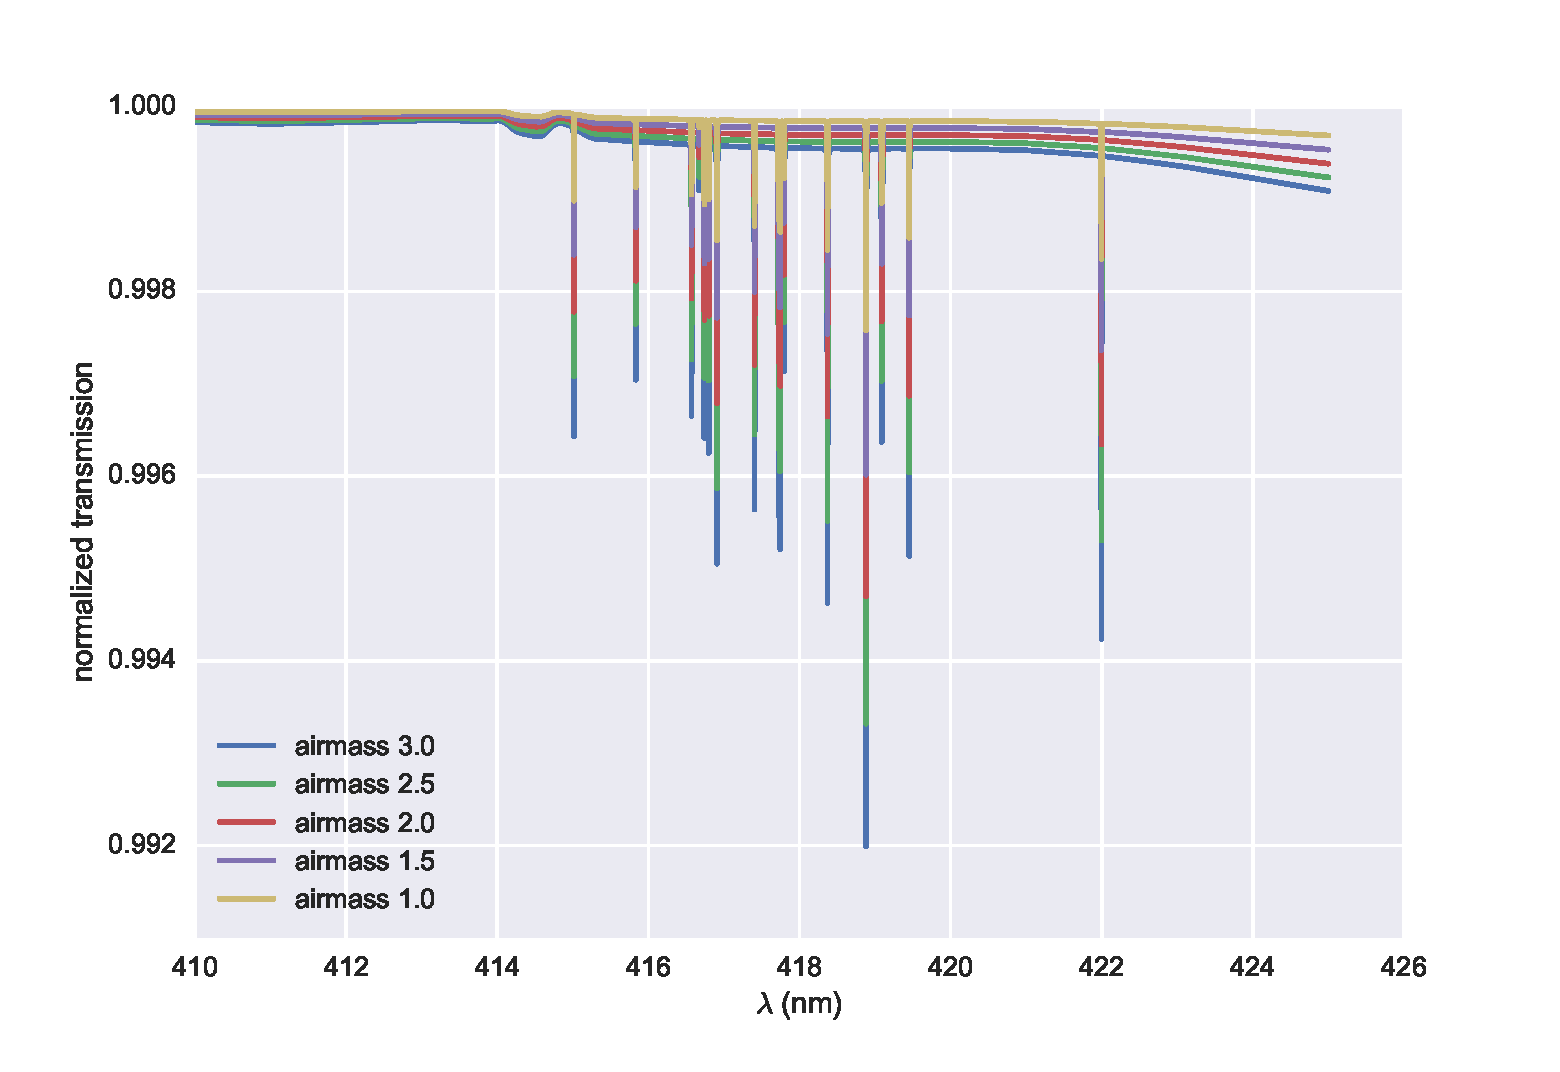
\includegraphics[width=0.75\paperwidth]{./Figures/spectra_stack}
\end{figure}

For now, these airmasses were just selected for 20mm of water vapor at the arbitrary test interval, $410-425$
nm. 

From the list of 50 randomly chosen airmasses, the binsize was increased in increments of 0.15 nm, starting at
the left and working right, for a total of 100 bins. For a given binsize, the average normalized flux and
standard deviation was calculated at each airmass to simulate variations as a function of time.
The results are summarized below, where a faint line corresponds to smaller binsize and bold to larger binsize.
\begin{figure}[H]
  \centering
  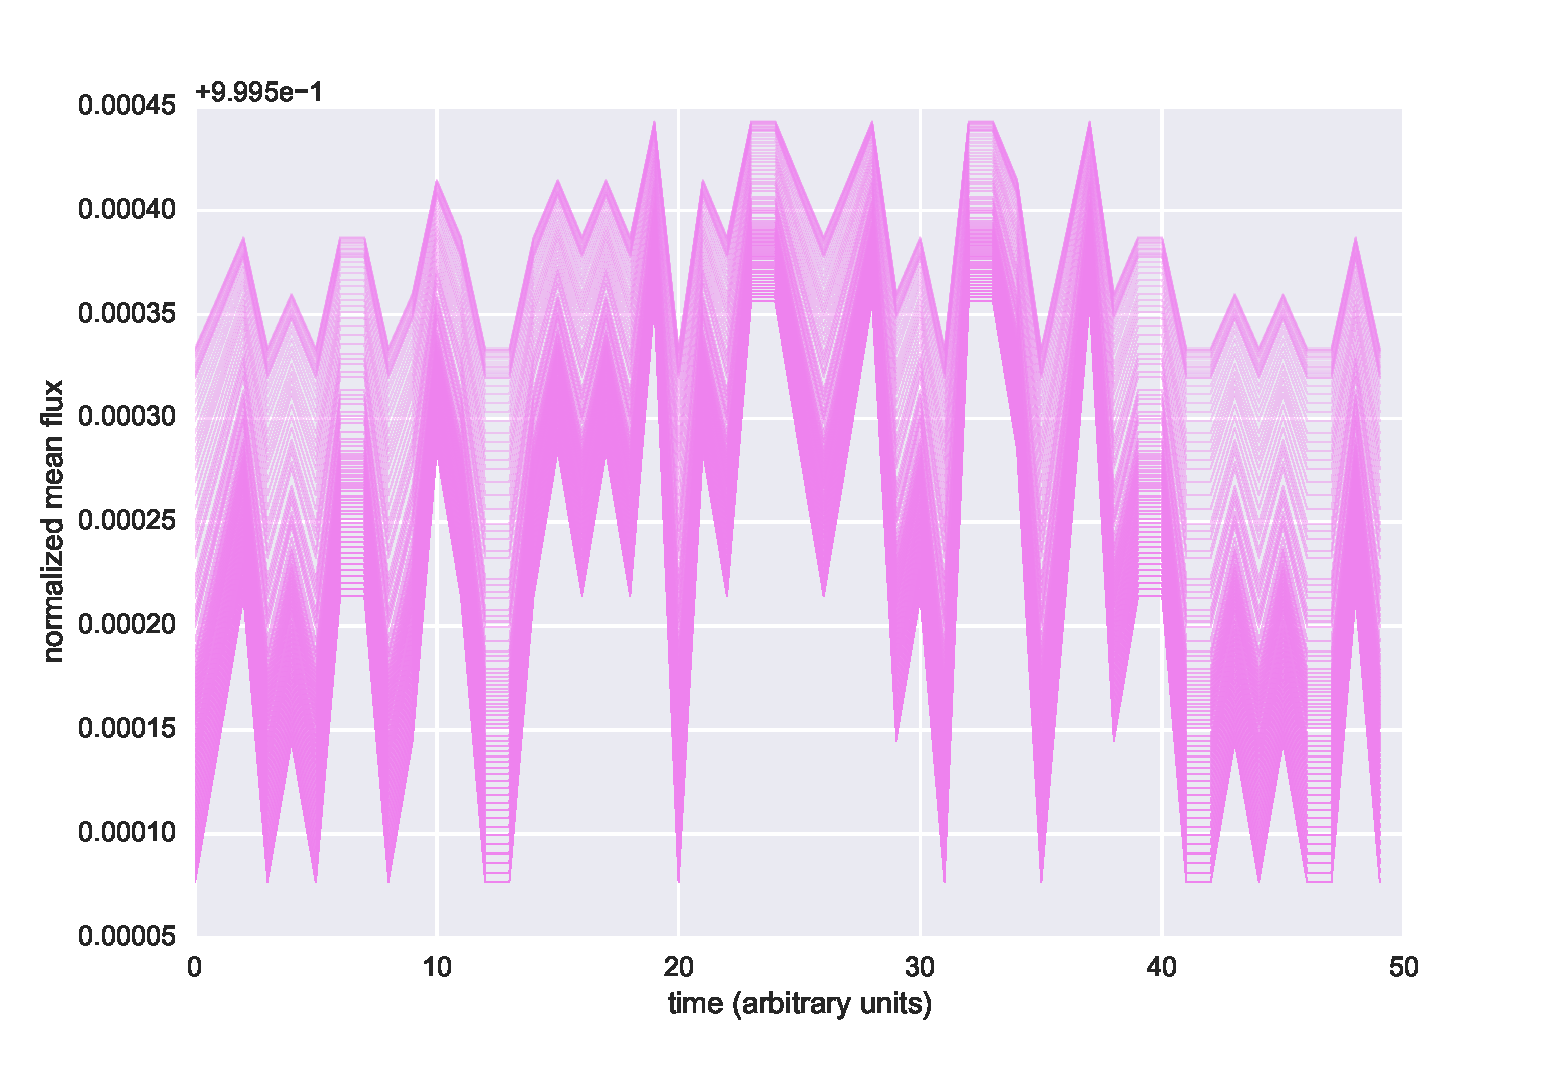
\includegraphics[width=0.75\paperwidth]{./Figures/meanflux_timeseries}
\end{figure}

\begin{figure}[H]
  \centering
  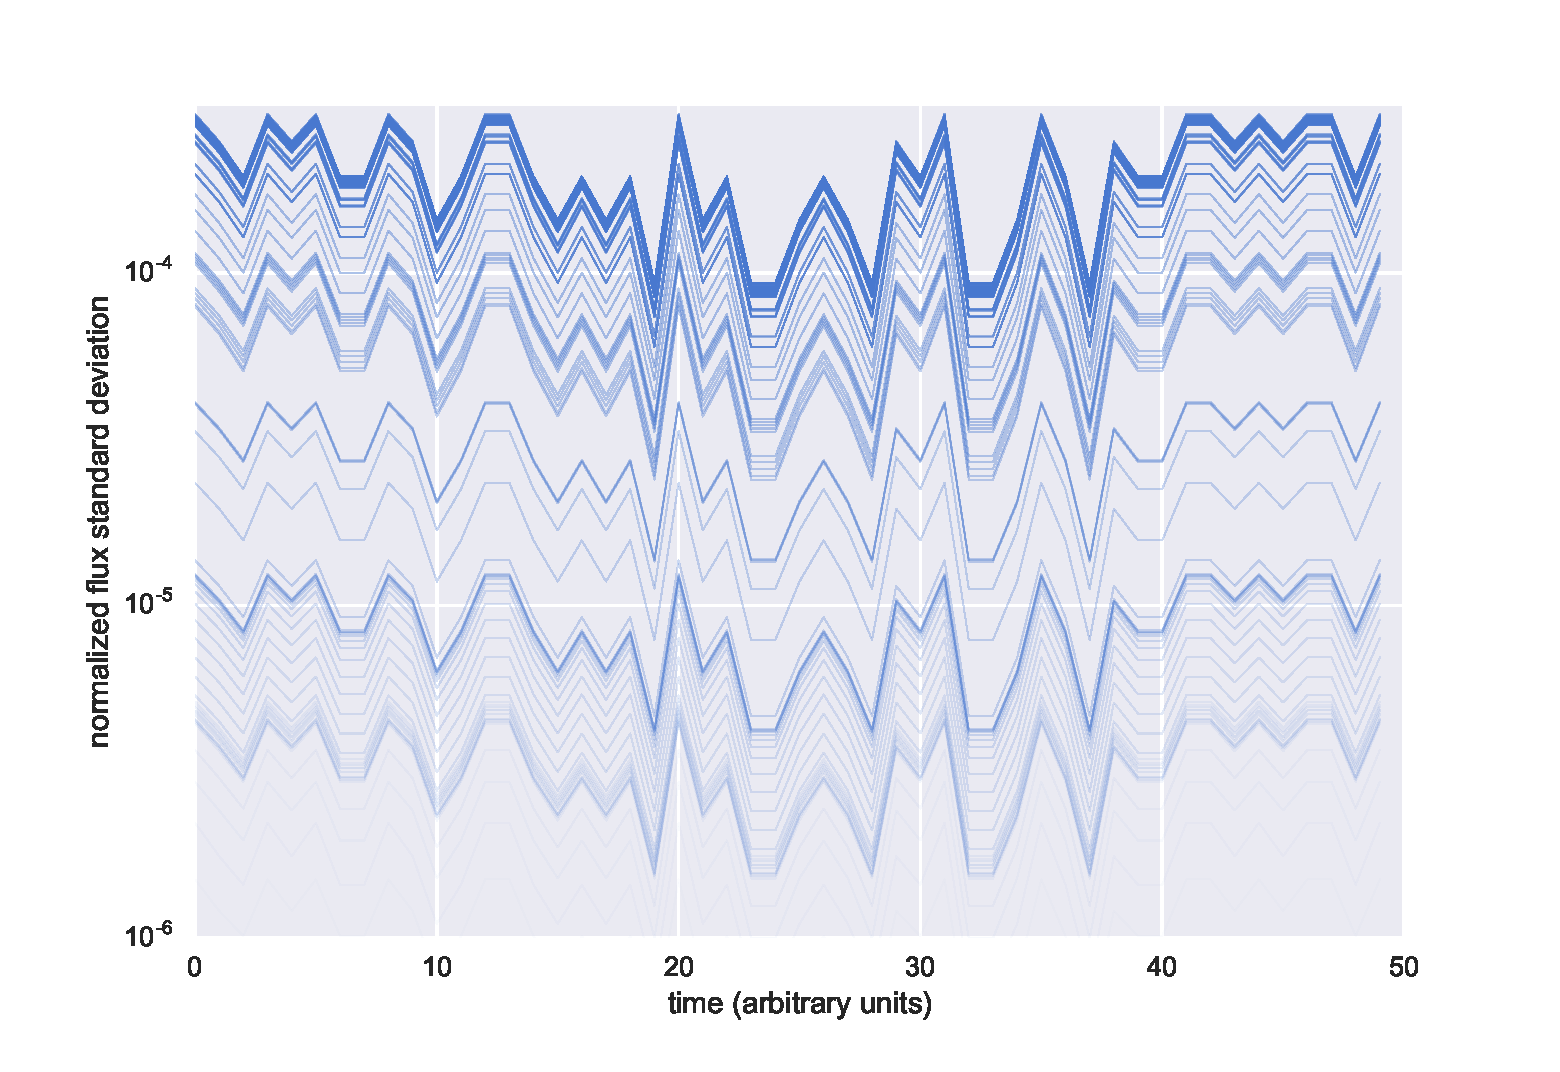
\includegraphics[width=0.75\paperwidth]{./Figures/stdev_timeseries}
\end{figure}



\end{document}
